%-------------------------------------
%        卒論のLaTeX用ひな形
%           制作 宮川ゼミ
%             2014/02
%-------------------------------------
\documentclass[uplatex,a4j,11pt]{jsarticle}
\usepackage{amsmath,amssymb,amsthm}
\usepackage{setspace}\setstretch{1.3}
\usepackage{calc}
\usepackage[textwidth=38zw, textheight=29\baselineskip+\topskip,heightrounded,dvipdfmx]{geometry}
\usepackage{okumacro}
\usepackage[yen]{jsverb}
\usepackage[dvipdfmx]{graphicx}
\usepackage{caption}
%\usepackage{natbib}
%\usepackage{bm,mathrsfs}

%--------   章,節  ----------------------------
\usepackage[medium,raggedright]{titlesec}

\newcommand{\sectionbreak}{\clearpage}%  章が変われば改ページ
% \newcommand{\subsectionbreak}{\vspace*{2\baselineskip}}%  節が変われば2行挿入

%--------   注(章末注で)  ---------------
\usepackage{endnotes}
\renewcommand{\footnote}{\endnote}     % footnote を endnote として使う
\renewcommand{\notesname}{章末注}
\renewcommand{\enotesize}{\normalsize}
\renewcommand{\theendnote}{\arabic{endnote}}
\renewcommand{\makeenmark}{\textsuperscript{\theenmark)}}

\makeatletter
% \def\enoteheading{\section*{\notesname % 修正前
\def\enoteheading{\subsection*{\notesname % 修正後:章末注は節として。章の一部なので。
  \@mkboth{\MakeUppercase{\notesname}}{\MakeUppercase{\notesname}}}%
  \mbox{}\par\vskip-\baselineskip}
\makeatother

%-----    定理   -----------------------
\newtheoremstyle{roman}% name
    {8pt}%        Space above
    {8pt}%        Space below
    {}%           Body font
    {}% Indent amount (e.g., empty, \parindent)
    {\bfseries}%  Thm head font
    {}%          Punctuation after thm head
    {0.8zw}%      Space after thm head (e.g., " ")
    {#1#2}%           Thm head spec (empty means `normal')
\theoremstyle{roman}
\newtheorem*{definition}{定義} 
\newtheorem{assumption}{仮定}
\newtheorem{proposition}{命題}
\newtheorem{theorem}{定理}

%------    証明   -------------------------
\newcommand{\prooffont}{\bfseries}
\renewcommand{\proofname}{\prooffont 証明\hspace{0.3zw}\nopunct}
\renewcommand{\qedsymbol}{(証明終)}
%%\newcommand{\noqed}{\renewcommand{\qedsymbol}{}}

\newcommand{\E}{\mathbb{R}}
\renewcommand{\le}{\leqslant}
\renewcommand{\leq}{\leqslant}
\renewcommand{\ge}{\geqslant}
\renewcommand{\geq}{\geqslant}
% \usepackage{accents}
% 	\newcommand{\ubar}[1]{{\underaccent{\bar}{#1}}}


%----- 傍点  ---------------------------------------
\makeatletter
\def\kenten#1{%
  \ifvmode\leavevmode\else\hskip\kanjiskip\fi
  \setbox1=\hbox to \z@{・\hss}%
  \ht1=.63zw
  \@kenten#1\end}
\def\@kenten#1{%
  \ifx#1\end \let\next=\relax \else
    \raise.63zw\copy1\nobreak #1\hskip\kanjiskip\relax
    \let\next=\@kenten
  \fi\next}
\makeatother
\newcommand{\bouten}{\kenten}	% 傍点

%-------   リンク,ブックマーク   ---------
\usepackage[dvipdfmx,bookmarkstype=toc=true,bookmarks=true,pdfpagemode=UseOutlines,
colorlinks=true,urlcolor=black,linkcolor=black,citecolor=black,linktocpage=true,%
pdfstartview=FitH,%
pdfpagelayout=OneColumn,bookmarksnumbered=true,bookmarksopen=true,%
pdfstartpage={}]{hyperref}
\providecommand*{\phantomsection}{}
\usepackage{pxjahyper}


\begin{document}
%----------------- 表紙 ---------------------
\newcommand{\kyo}{{\number\year}年{\number\month}月{\number\day}日}
\newcommand{\提出日}{\kyo}
%---各自記入-----------
\newcommand{\題目}{権力分立の堅牢性}
\newcommand{\副題}{ゲーム理論による分析}
\newcommand{\学番}{1762247E}
\newcommand{\氏名}{山本 燿司}
%-----------------------
\thispagestyle{empty}
\begin{flushright}
{\Large \提出日 提出}\\[0.2\textheight]
\end{flushright}
\begin{center}
% {\Large 研究指導論文要旨}\\[2\baselineskip]  % 要旨の表紙で必要
{\Large \hspace{1zw}\Huge \題目}\\[\baselineskip]
{\Large \——\副題\——} %副題があれば
\end{center}
\vfill

\begin{flushleft}
\hspace{25zw}{\Large 宮川栄一研究室}\\[1zh]
\hspace{25zw}{\Large 学籍番号\ \学番}\\[1zh]
\hspace{25zw}{\Large 氏名\hspace{0.5zw}\氏名}
\end{flushleft}
\clearpage

%--------    目次     ---------------
\thispagestyle{empty}
\tableofcontents
\thispagestyle{empty}
\clearpage

%--------   本文   -----------------
\section*{序章}
\addcontentsline{toc}{section}{序章}
\setcounter{page}{1}

% \subsection*{研究動機}
\begin{itemize}
  \item 中学・高校の教科書には、三権分立しているから大丈夫(国家権力の暴走は防がれている)とある。政治学の教科書にもそうある(?)
  \item モンテスキューに遡っても、ルソーに遡っても、「こういうふうに分立したら大丈夫」とあるが、その理由やメカニズムは明らかになっていない。
  \item 今回見たいのは、各国家権力それぞれが暴走する可能性のある中、どのようなメカニズムでその暴走が防がれているのかという点。
  \item この観点での、既存論文はxxx。
\end{itemize}




\section{モデル}

プレイヤーが$N=\lbrace 内閣, 国会 \rbrace$の、2期間の不完備情報動学ゲームを考える。



司法を入れない理由は2つある。1つは、xxx。司法の違憲判決は行政執行や法律制定の数年から数十年に出される。
例として、旧優性法、足尾銅山。(TODO:他の例や、反対にすぐに政策が違憲/違法判定された例を調べる)。
その頃には、別の政権・議席割合であり、別のゲームをしていると考えるのが妥当。
2つ目は、見たかった司法の暴走の例は人質司法だが、これは政策決定とは別のゲームをしてる(司法の役割は、違法/違憲と合法/合憲の境目をはっきりさせる)。


国会の効用関数を以下のように定義する。
$$u_\text{国会} = v_t(\;W\;,\; a_\text{国会}\;) × \delta^{t-1}_\text{市民}$$
$v_t(\;W\;,\; a_\text{国会}\;)$は、国民(以下、"市民"とする)の厚生関数である。この厚生関数は、世界の状態である$W=\lbrace 有事, 平時\rbrace$と、国会が承認する政策$a_{国会}=\lbrace A, B\rbrace$によって決まる。
有事では改革的政策$A$が長期的がより効果的であり、平時では保守的政策$B$(TODO:命名を変える。平時で有効+短期的な利得があるという意味。)がより効果的であるとする。
時間割引率$\delta_{市民}=\lbrace \delta_L, \delta_H \rbrace, \delta_L<\delta_H$は、主権である市民が愚民($\delta_L$)であるか、賢民($\delta_H$)であるかを表している。

内閣の効用関数を以下のように定義する。
$$ u_\text{内閣} =\;\; \lbrace T\lbrace \alpha a_\text{国会} + \beta (1-a_\text{国会}) \rbrace  + (1-T)v_t(\;W\;,\; a_\text{国会}\;) \rbrace × \delta^{1-t}_{内閣}$$
内閣も市民の一人であるので、厚生関数$v_t(\;W\;,\; u_\text{国会}\;)$を同じように持つ。ただし、$a_{国会}=\lbrace A, B\rbrace = \lbrace 1,0\rbrace$とする。
加えて、内閣には私欲とも呼ばれる独自の正義感があり、各政策を実行すること自体からも効用を得る。それぞれ、改革的政策Aから得られる効用を$\alpha$, 保守的政策Bから得られる効用を$\beta$とする。
この私欲と公共心の割合は$T:(1-T)$で表される。ただし、$T\in[0,1]$ 。

国会は、市民から直接声を聞くため市民の時間割引率$\delta_{市民}$を観測できるが、内閣は観測できないものとする。

反対に、内閣は自身の私欲と公共心の割合$T:(1-T)$に加え、外交や調査機関の情報\footnote{これらはモデル外の話。}から世界の状態$W=\lbrace 有事, 平時\rbrace$を観測できるが、国会からは観測できないものとする。


\subsection*{市民の厚生関数$v_t(\;W\;,\; a_\text{国会}\;)$における仮定}

有事における政策$A$によるt期の効用を$v'_{At}$とし、平時における政策$A$によるt期の効用を$v_{At}$とする。

世界の状態$W$が有事であっても平時であっても、保守的政策$B$の効用は変わらないものとする。
また前述の通り、有事では改革的政策$A$が長期的にはより効果的であり、平時では保守的政策$B$が長期的により効果的である。よって以下の仮定を得る。
\begin{assumption}  $v_{A1} + v_{A2}<v_{B1} + v_{B2} <  v_{A1} + v'_{A2}$ \end{assumption}


また、改革的政策$A$は実行に時間がかかるため、1期目における効用は平時でも有事でも変化がないが、2期目においてその効果が出るものとする。
さらに、平時または有事における各期の効用の大小関係、及び、平時と有事間での$A$政策の2期目の効用の差分と、$B$政策の1期目と2期目の差分の大小関係を以下のように仮定する。
\begin{assumption}  $v_{A1} < v_{B2} < v_{A2} < v_{B1} < v'_{A2}$  \end{assumption}
\begin{assumption}  $v_{A2} - v_{B1} < v'_{A2} - v_{B2}$  \end{assumption}

以下の図1はこれらの仮定を含めたものである。
\begin{figure}[htbp]
  \centering
  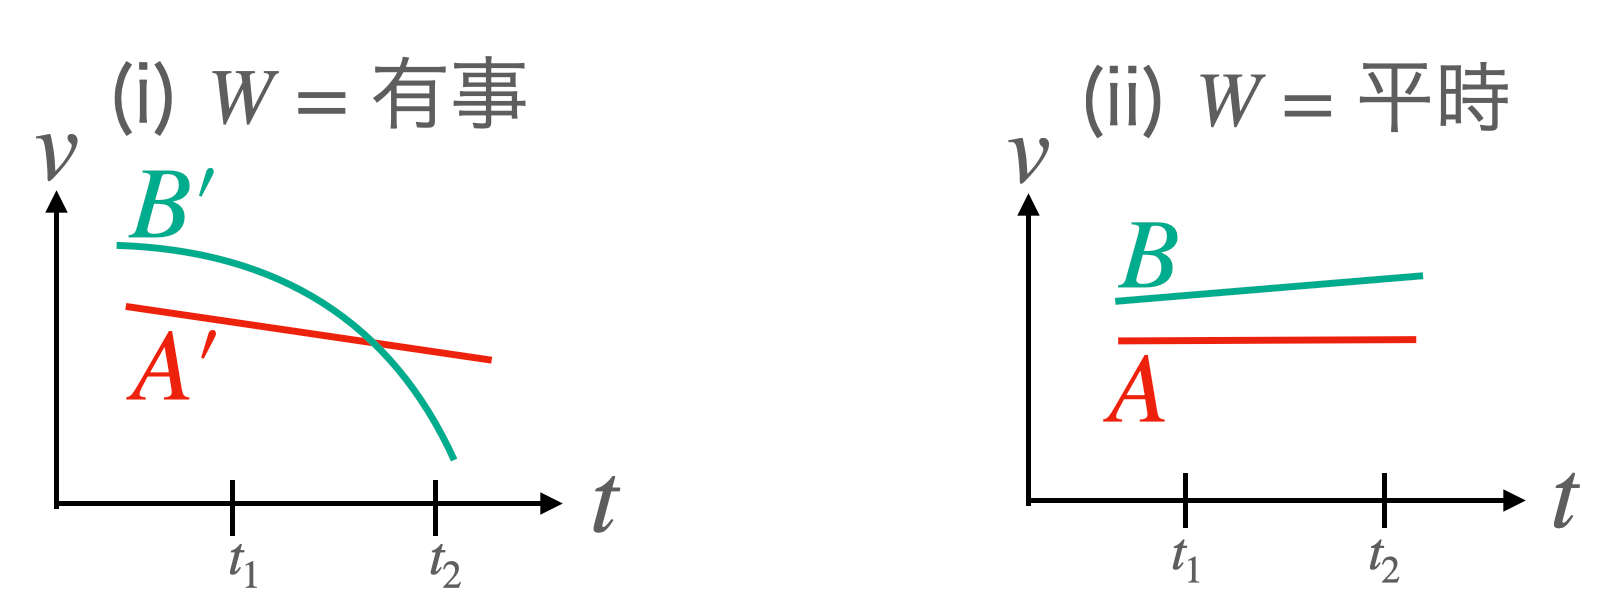
\includegraphics[width=0.7\textwidth]{./image/assumption_welfare_policy.png}
  \caption{厚生関数の仮定} 
  \label{fig:assumption_welfare_policy}
\end{figure}


\subsection{国会の最適反応}

\subsection{内閣の最適反応}



\theendnotes %章末注
\section{均衡}

注がある章の末尾にはコマンド \verb#\theendnotes# を挿入すべし\footnote{章末注は節として扱います。}。


\theendnotes %章末注
\section{終章}

一二三四五六七八九十一二三四五六七八九十一二三四五六七八九十一二三四五六七八九十一二三四五六七八九十一二三四五六七八九十一二三四五六七八九十一二三四五六七八九十一二三四五六七八九十一二三四五六七八九十一二三四五六七八九十一二三四五六七八九十一二三四五六七八九十一二三四五六七八九十一二三四五六七八九十一二三四五六七八九十


\section*{謝辞}
\addcontentsline{toc}{section}{謝辞}
三島大輝君の卒論ファイルを参考にしました。三島君は濱田高彰君のファイルを参考にしたそうです。先輩の知恵に感謝します。

\newpage
\addcontentsline{toc}{section}{参考文献}
\begin{thebibliography}{99}
%------------------------------

\item ロバート・ギボンズ (1995) 『経済学のためのゲーム理論入門』
(福岡正夫・須田伸一訳)創文社。

\item 高須賀義博 (1994) 「再生産の局面分析」『経済研究』第25巻第3号,
18--27頁。

\item Moulin, H. (1983), \emph{The Strategy of Social Choice}, Amsterdam, Netherlands:
North-Holland.

\item Moore, J., and R. Repullo (1990), ``Nash Implementation: A Full Characterization,''
\emph{Econometrica}, Vol.\ 58, No.\ 5, pp.\ 1083--1099.

%-----------------------
\end{thebibliography}
\end{document}